\documentclass[10pt,sans,english,compress,xcolor=dvipsnames]{beamer}
\author[Lily ]{ Dr Lily Asquith (Lily, she/her)}

\usetheme{Szeged}
%\defbeamertemplateparent{enumerate items}{enumerate item,enumerate subitem,enumerate subsubitem,enumerate mini template}
\definecolor{titcol}{RGB}{16,78,100} 
\setbeamercolor{frametitle}{fg=titcol,bg=White}
\useoutertheme{miniframes} 
\useinnertheme{rectangles}

\usepackage{pifont}
\newcommand{\tick}{\textcolor{grn}{\ding{52} } }
\newcommand{\nope}{\textcolor{red}{\ding{54} } }


\usepackage{soul}
\usepackage{cancel}

\usepackage[most]{tcolorbox}
\definecolor{LilyBlack}{rgb}{0.05,0.1,0.3} % UBC Blue (primary)
\usecolortheme[named=LilyBlack]{structure}

\usepackage{booktabs}
\usepackage{tabularx}
%\usepackage{tikz}
%\def\checkmark{\tikz\fill[scale=0.4](0,.35) -- (.25,0) -- (1,.7) -- (.25,.15) -- cycle;}

\usepackage{physics}

\usepackage{xparse}

\setbeamertemplate{footline}{%
  \leavevmode%
  \hbox{\begin{beamercolorbox}[wd=.5\paperwidth,ht=2.5ex,dp=1.125ex,leftskip=.3cm plus1fill,rightskip=.3cm]{author in head/foot}%
    \usebeamerfont{author in head/foot}\insertshortauthor
  \end{beamercolorbox}%
  \begin{beamercolorbox}[wd=.5\paperwidth,ht=2.5ex,dp=1.125ex,leftskip=.3cm,rightskip=.3cm plus1fil]{title in head/foot}%
    \usebeamerfont{title in head/foot}\insertshorttitle\hfill\insertframenumber\,/\,\inserttotalframenumber
  \end{beamercolorbox}}%
  \vskip0pt%
}

\DeclareMathSizes{10}{10}{6}{4} % this one
%\DeclareMathSizes{10.95}{10}{6}{4}   % For size 10 text

\newcommand*\ColorBox[3][black]{%
  \makebox[2em][c]{%
    \setlength\fboxsep{-.5\fboxrule}%
    \raisebox{\dimexpr-#3em+.5ex}{%
      \fcolorbox{#1}{#2}{%
        \rule{0pt}{\dimexpr#3em*2}%
        \rule{\dimexpr#3em*2}{0pt}%
      }%
    }%
  }%
}

\usepackage{hyperref}
\hypersetup{
    colorlinks=true,
    linkcolor=blue,
    filecolor=magenta,      
    urlcolor=blue,
    pdftitle={Overleaf Example},
    pdfpagemode=FullScreen,
    }

\urlstyle{same}

% this part excludes specified frames from counters in navigation bar
\makeatletter
\let\beamer@writeslidentry@miniframeson=\beamer@writeslidentry
\def\beamer@writeslidentry@miniframesoff{%
  \expandafter\beamer@ifempty\expandafter{\beamer@framestartpage}{}% does not happen normally
  {%else
    % removed \addtocontents commands
    \clearpage\beamer@notesactions%
  }
}
\newcommand*{\miniframeson}{\let\beamer@writeslidentry=\beamer@writeslidentry@miniframeson}
\newcommand*{\miniframesoff}{\let\beamer@writeslidentry=\beamer@writeslidentry@miniframesoff}
\makeatother


\makeatletter
\newcommand\notsotiny{\@setfontsize\notsotiny{6.5}{7.5}}
\makeatother




\usepackage{multicol}
\usepackage{sansmath}
\usepackage{minted}
\definecolor{LightGray}{gray}{0.95}
\usepackage{nicematrix}
%\usepackage{statmath}
\usepackage{cancel}
\newcommand<>{\xxcancel}[1]{\alt#2{ \textcolor{red}{\cancel{#1}}\vphantom{#1} }{#1}}
\usepackage{tikz}

\usepackage{array}
\newcolumntype{L}{>{$}l<{$}}


\title[Maximum Likelihood Estimation]{Maximum Likelihood}
\date{}
\titlegraphic{
%\center

\includegraphics[scale=0.15]{sussex-logo}
}
% Lily includes for font and spacing
\usepackage{cmbright} % pretty nice but maybe a bit too different
\renewcommand{\baselinestretch}{1.1} 
\usepackage{sansmath}
% Lily highlight numerical answers for quicker marking
\usepackage{xcolor}
\definecolor{mygreen}{RGB}{226,254,226}
\definecolor{mylblue}{RGB}{205, 248, 250}
\definecolor{mylpink}{RGB}{159, 43, 104}
\usepackage[most]{tcolorbox}

\newtcbox[auto counter]{\ghl}
{enhanced, on line, boxsep=0pt,left=6pt,right=6pt,top=2pt,bottom=2pt,rightrule=1pt,
colback=mygreen,
colframe=black 
}
\newtcbox[auto counter]{\bhl}
{enhanced, on line, boxsep=0pt,left=6pt,right=6pt,top=2pt,bottom=2pt,rightrule=1pt,
colback=mylblue,
colframe=black 
}
\newtcbox[auto counter]{\yhl}
{enhanced, on line, boxsep=0pt,left=2pt,right=2pt,top=1pt,bottom=1pt,rightrule=1pt,
colback=lyellow,
colframe=black 
}

\newcommand{\bhlm}[1]{\bhl{$#1$}}

\newtcbox[auto counter]{\phl}
{enhanced, on line, boxsep=0pt,left=6pt,right=6pt,top=2pt,bottom=2pt,rightrule=1pt,
colback=mylpink,
colframe=black 
}

\DeclareMathOperator*{\plim}{plim}
\begin{document}

\newcommand\info{\mathcal{J}_{\theta}}
\newcommand\loglike{\ln{ \mathcal{L}_{\theta}} }
\newcommand\like{\mathcal{L}_{\theta} }

\newcommand\thetahat{\hat{ \theta }  }

\definecolor{grn}{RGB}{0,128,0} 
\newcommand{\gbl}[1]{\textcolor{grn}{#1}}

\definecolor{wh}{rgb}{0.95, 0.95, 0.96}
\newcommand{\wht}[1]{\textcolor{wh}{#1}}

%\newcommand{\inprob}{\overset{p}{\to}}

\newcommand{\boo}[1]{\textbf{\textcolor{red}{#1}}}

\newcommand{\covmat}{\mathbf{\textcolor{magenta}{\Sigma}} }


\definecolor{purr}{RGB}{128,0,128} 
\newcommand{\purp}[1]{\textcolor{purr}{#1}}

\newcommand{\magt}[1]{\textbf{\textcolor{magenta}{#1}}}
 \newcommand{\magtn}[1]{\textcolor{magenta}{#1}}
 
%\definecolor{bbl}{RGB}{128,0,128} 
\newcommand{\bbl}[1]{\textcolor{blue}{#1}}

\newcommand{\rbl}[1]{\textcolor{red}{#1}}

\definecolor{dblu}{RGB}{37,150,190} 
\newcommand{\blu}[1]{\textcolor{dblu}{#1} }

\definecolor{dor}{RGB}{255,40,0} 
\newcommand{\dor}[1]{\textcolor{dor}{#1} }

\definecolor{darkgreen}{RGB}{46,139,87} 
\newcommand{\dgreen}[1]{\textbf{\textcolor{darkgreen}{#1}} }
%\newcommand{\gbl}[1]{\textcolor{darkgreen}{#1}}

\definecolor{lgray}{RGB}{222,222,222} 

\definecolor{lyellow}{RGB}{255,255,224} 

\newcommand{\E}[1]{\mathbf{E}_{#1}}
%
\newcommand{\rvX}[1]{X_{(#1)} } 

\newcommand{\rvY}[1]{Y_{(#1)} }

\newcommand{\rvx}[1]{x_{(#1)} } 

\newcommand{\rvy}[1]{y_{(#1)} }



\newcommand{\red}[1]{\textcolor{red}{#1} }

\newcommand{\bluedots}{\blu{\ldots} }

\newcommand{\dordots}{\dor{\ldots} }


\newcommand{\where}{\dgreen{\;where\;} }


\newcommand{\pand}{\dgreen{\;and\;} }
\newcommand{\por}{\dgreen{\;or\;} }

\newcommand{\sumN}{ \sum\limits_{\blu{i}}^{\blu{N}} }

\newcommand{\sumZ}{ \sum\limits_{\dor{j}}^{\dor{Z}} }

\newcommand{\Expec}[1]{ \mathbb{E}[#1] }


\newcommand{\Xfj}[1]{ X_{ \dor{#1} } }

\newcommand{\xfi}[1]{ x_{ \blu{#1} } }

\newcommand{\Xij}[2]{ X_{\mage{#1},\blu{#2} }}

\newcommand{\sumxi}{ \sumN \xfi{i} }

\newcommand{\sumXj}{ \sumZ \Xfj{j} }

\newcommand{\sumZa}[1]{ \sumZ {#1}_{ \dor{j} } }

\newcommand{\sumZab}[2]{ \sumZ {#1}_{ \dor{j} }\, {#2}_{ \dor{j} } }

\newcommand{\sumNab}[2]{ \sumN {#1}_{ \blu{i} }\, {#2}_{ \blu{i} } }

\newcommand{\vecxi }{ [ \xfi{1} \xfi{2}, \bluedots, \xfi{N} ] }

\newcommand{\vecXj }{ [ \Xfj{1} \Xfj{2}, \bluedots, \Xfj{Z} ] }

\newcommand{\vecXij }{ [ \Xij{1}{1} \Xij{1}{2}, \bluedots, \Xij{1}{N_1} ],\, [ \Xij{2}{1} \Xij{2}{2}, \bluedots, \Xij{2}{N_2} ],\, \dordots,\,[ \Xij{Z}{1} \Xij{Z}{2}, \bluedots, \Xij{Z}{N_Z} ] }

% definitions

\newcommand{\overNblack}{ \dfrac{1}{N} }
\newcommand{\overN}{ \dfrac{1}{ \blu{N} } }

\newcommand{\defmean }{ \overline{x} = \overN \sumN \xfi{i} }

\newcommand{\meanx }{ \overline{x} }
\newcommand{\meansqx }{ \overline{x^2} }
\newcommand{\sqmeanx }{ \overline{x}^2 }
\newcommand{\devsq}{ (\xfi{i} - \meanx)^2 }

%\newcommand{\var }[1]{ \mathcal{V}_{#1} }
\newcommand{\defvar }{ \var{x} = \overN \sumN \devsq }
\newcommand{\defvarshort }{ \var{x} = \meansqx - \sqmeanx }

\newcommand{\defstd }{ s_x = \sqrt{ \var{x} }  }

\newcommand{\defwmean }{ \overline{X} = \dfrac{ \sumZab{w}{X} }{ \sumZa{w} } }  

\newcommand{\defw }{ w_{\dor{j}} = \dfrac{1}{ \var{\Xfj{j} } } }



\begin{frame}
\titlepage
\end{frame} 

\section*{Preamble}




% contents
\begin{frame}{Maximum Likelihood Estimation}
\small
\begin{itemize}
\item Some simple examples of the most likely parameter value
\item Estimating multiple parameters 
\item Estimator Bias and Mean Squared Error
\item The Score, Information, and Minimum Variance Bound
\item The Graphical Method
\item First look at Likelihood Ratio and Wald test
\end{itemize}

\end{frame} 

%\begin{frame}{Naive Bayes}
%\footnotesize
%
%MLE also used to train Neural Networks : loss function is often negloglike\\[1ex]
%Transformers
%Gaussian Mixture models, Hidden Markov models, also apparently use MLE.\\[1ex]
%
%
%\end{frame}


\begin{frame}{Intro, reminder of big picture}
\footnotesize
Maximum Likelihood Estimation is arguably the most important concept for Machine Learning.\\[1ex]
%I can't think of a ML algorithm that doesn't relate to MLE in some way or other.\\[1ex]
 Parameter estimation in theory is sold as trying to find the value of a mean, or a rate, or similar.\\[1ex]
 In practical data science problems, a parameter might be a class with a few possible labels, or a binary yes/no. Choosing the parameter value which is the most likely one is unsurprisingly, always the best choice!\\[1ex]
\end{frame} 

\begin{frame}{Parameter Estimation}
\footnotesize
%According to the data, which parameter value is most probable?\\[1ex]

%Note that in the Machine Learning world, we often use `class' rather than parameter, when we are trying to classify data.\\
Reminder of some \bbl{Model} \magtn{Parameters}:\\[1ex]

$K \sim \bbl{Bernoulli(\magtn{p})}$ The parameter $\magtn{p}$ is the probability of success\\ \texttt{bernoulli(p=p)}.\\[2ex]
$K \sim \bbl{Binom(\magtn{n,p})}$ Two parameters, $\magtn{n}$ is the number of Bernoulli trials\\ \texttt{binom(p=p,n=n)}.\\[2ex]
%$K \sim Poisson(\magtn{\lambda})$ The parameter $\lambda$ is count/time. The RV $K$ is the number of successes.\\
$X\sim \bbl{Uniform(\magtn{a,b})}$ Two parameters $\magtn{a, b}$ are the bounds of the support\\ \texttt{uniform(loc=a, scale=b-a)}.\\[2ex]
$X\sim \bbl{Expon(\magtn{\lambda})}$ The parameter $\magtn{\lambda}$ is rate\\ \texttt{expon(scale=1/$\lambda$)}.\\[2ex]
%$X\sim Beta(\alpha, \beta)$ The (hyper)parameters $\alpha, \beta$ provide the shape.\\
$X\sim \bbl{Norm}(\magtn{\mu, \sigma})$ Two parameters $\magtn{\mu}$ is the mean, and $\magtn{\sigma}$ is the standard deviation.\\ \texttt{norm(loc=mu,scale=sigma)}.\\[2ex]

\end{frame} 



\section*{Binomial $\hat{p}$}


\begin{frame}{Estimating Binomial $\magtn{p}$}
\footnotesize
According to the data, which value of $\magtn{p}$ is most probable?\\[1ex]

Back to tossing a coin!  We find $k$ heads in $n$ tosses. Let's Estimate the probability of a tossed coin landing heads up, $\magtn{p}$.\\

Binomial PMF: $p_K(k) = C_k^n \magtn{p}^k (1-\magtn{p})^{n-k}$ \bbl{Note that $p_K(k)$ is the PMF: the probability of $k$ heads.}\\[1ex]

We can write this PMF as a conditional Probability:\\
$P(k | \magtn{p}) = C_k^n \magtn{p}^k (1-\magtn{p})^{n-k}$\\[1ex]

We might as well remind ourselves of the form of $C_k^n = \dfrac{n!}{k!(n-k)!}$. I am happy to note that this does not depend on the parameter $\magtn{p}$ (it is just a number).\\

\end{frame} 



\begin{frame}{Visual Reminder of Binomial PMF}
\footnotesize

\begin{center}
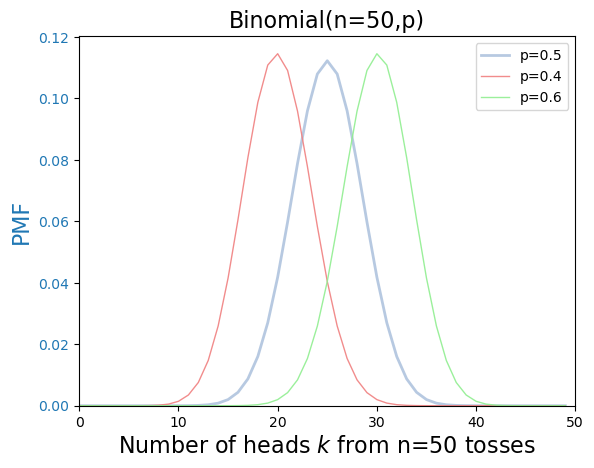
\includegraphics[scale=0.38]{BinomLikeIntro.png}
\end{center}
These plots show the Binomial PMF under different assumptions for our parameter $\magtn{p}$. The data we measure is $k$. As we can see, a given measure of $k$ can be consistent with a range of potential $\magtn{p}$. We want to know, given $k$, what is the most likely $\magtn{p}$?
\end{frame} 


\begin{frame}{Estimating Binomial $\magtn{p}$}
\footnotesize
The most likely \magtn{p} is our \bbl{Maximum Likelihood Estimate} (MLE) for \magtn{p}:  \bbl{$\hat{p}$}.\\[1ex]

$p_K(k) = P(k | \magtn{p}) = C_k^n \magtn{p}^k (1-\magtn{p})^{n-k}$\\[1ex]

I toss the coin $n=50$ times and observe $k=27$ heads. \\
$\mathcal{L}_{p} = P(k=27 | \magtn{p}) = C_k^n \magtn{p}^{27} (1-\magtn{p})^{23}$\; (\bbl{Note $N=1$, so $\mathcal{L}_{p} = \prod\limits_i^N p_K = p_k$})\\[1ex]
 
To maximise the Likelihood, we take the derivative \magtn{with respect to p} and set it to zero, solving for \bbl{$\hat{p}$}.\\

 $\dfrac{d}{d\magtn{p}} ( C_k^n\, \magtn{p}^{27} (1-\magtn{p})^{23} )= 
C_k^n
\left(
 27 \magtn{p}^{26} (1-\magtn{p})^{23} - \magtn{p}^{27} 23(1-\magtn{p})^{22} 
 \right) =0$\\[1ex]
 % $27 \magtn{p}^{26} (1-\magtn{p})^{23} = \magtn{p}^{27} 23(1-\magtn{p})^{22}$\\[1ex]
% 
 We cancel factors of $\magtn{p}$ and $1-\magtn{p}$ to find  ... $\bbl{\hat{p} = \dfrac{27}{50}}$. Not very surprising :)

\end{frame} 

% 
% 
% 
% #from scipy.special import binom as bnc
% # bnc(50,28) 
% #88749815264600.02
% # 

\defverbatim[colored]\badLike{
\begin{minted}[bgcolor=LightGray]{python}
0.5**(5e3) # 0.0
0.5**(1e3) # 9.332636185032189e-302
\end{minted}
}

\defverbatim[colored]\goodLog{
\begin{minted}[bgcolor=LightGray]{python}
0.5*(5e3) # 2500
\end{minted}
}


\begin{frame}[fragile]{Log Likelihood}

\footnotesize
Logs are very useful because eg \ghl{$\ln{(abc)} = \ln{a} + \ln{b} + \ln{c} $} \\[1ex]

Consider a simple machine learning problem where there is a flat probability of $p_K(k) =0.5\,f(\theta)$ and $N=5\times10^3$ data measurements. \\[1ex]
\begin{columns}
\begin{column}{0.0001\textwidth}
\vspace*{70pt}
\end{column}
\begin{column}{0.9998\textwidth}
\only<1>{
\bbl{The Likelihood is $\mathcal{L}_{\theta} = \prod\limits_i^N p_K(k)$:}\\[1ex]
$\mathcal{L}_{\theta} = \prod\limits_i^{N} 0.5\,f(\theta) = (0.5\,f(\theta))^{5\times10^3}$ \magtn{uh-oh!}. \\[1ex]

\badLike

\magtn{The Likelihood is not appropriate for numerical computations unless the dataset is really small. And we like big datasets.} \\[1ex]
}
\only<2>{

\bbl{The Log Likelihood is}:\\
$\ln {\mathcal{L}_{\theta} } = \sum\limits_i^{N} 0.5\,f(\theta) = (5\times10^3)(0.5\,f(\theta))$ \\

\goodLog

\magtn{The numerical manageability of logs is not the only reason for using them, but is a compelling one.}\tick
}
\end{column}
\begin{column}{0.0001\textwidth}
\vspace*{70pt}
\end{column}
\end{columns}
\end{frame}



\begin{frame}{Log Likelihood for Coin Toss}
\footnotesize
Reminder: we toss a coin 50 times, see 27 heads. This is a single Binomial probability measurement ($N=1$), so $\like = p_k$.\\[1ex]

$\ln \mathcal{L}_p = \ln p_K = \ln \left(C_{_{27}}^{^{50}} p^{27} (1-p)^{23}\right) = \ln \left( C_{_{27}}^{^{50}}\right) +  27 \ln{ (p)} + 23 \ln{ (1-p)}$\\[1ex]

$\dfrac{d}{dp} \ln \mathcal{L}_p  = 0 + \dfrac{27}{p} - \dfrac{23}{(1-p)} = 0$\;\;\; \bbl{* chain rule}\\[3ex]

\bbl{$\hat{p} =  \dfrac{27}{50}$} as before. We don't lose any information by using the log.\\[2ex]

\notsotiny
\bbl{* Chain rule: $f(g) = \ln g$ and $g(\theta) = \like$, so $\dfrac{\partial f(g(\theta))}{\partial \theta} = \dfrac{\partial \ln g}{\partial g}\dfrac{\partial \like}{\partial \theta} = \dfrac{1}{g}\dfrac{\partial \like}{\partial \theta} =  \dfrac{1}{\like}\dfrac{\partial \like}{\partial \theta} $} \\[1ex]
\end{frame}


\section*{Expon $\hat{t}$}

\begin{frame}{Most Likely Taxi Waiting Time}
\footnotesize
To estimate the parameter for a continuous RV, we use the PDF rather than the PMF in the binomial example.\\

The Exponential PDF is $f_T(t;\lambda) = \lambda e^{-\lambda t}$ We use this to model the waiting time t when the rate is $\lambda$, with expected value $1/T$.\\

\magtn{Data: three days in a row I get a taxi. My waiting times are 15, 18, 11 minutes.}\\

We want to estimate $\lambda$ from these three data points. Let's write down the Likelihood:\\[1ex]% for these independent RVs $T = \{ T_{(1)}, T_{(2)}, T_{(3)} \}$:\\[1ex]

\bbl{The Likelihood is $\mathcal{L}_{\theta} = \prod\limits_i^N p_K(k)$:}\\[1ex]

$\mathcal{L}_{\lambda}  = (\lambda e^{ -\lambda \magtn{t_{(1)}} })  (\lambda e^{-\lambda \magtn{t_{(2)}} }) (\lambda e^{ -\lambda \magtn{t_{(3)}} })=\lambda^{\magtn{3}} e^{-\lambda( \magtn{t_{(1)} + t_{(2)} + t_{(3)}} ) } $


\end{frame}



\begin{frame}{Most Likely Taxi Waiting Time}
\footnotesize
\magtn{Data: three days in a row I go to wait for a taxi. My waiting times are 15, 18, 11 minutes.}\\

$\mathcal{L}_{\lambda}  = \lambda^3 e^{-\lambda(\magtn{ t_{(1)} + t_{(2)} + t_{(3)} }) } = \lambda^{\magtn{3}} e^{-\magtn{44}\lambda}$\\

$ \ln{\mathcal{L}_{\lambda} } = \ln{ ( \lambda^{\magtn{3}})}  - \magtn{44} \lambda = \magtn{3} \ln{ \lambda}  - \magtn{44} \lambda  $\\

$\dfrac{d}{d\lambda}  \ln \mathcal{L}_{\lambda}   = \dfrac{\magtn{3}}{ \lambda}  - \magtn{44} $\\
 
$\bbl{\hat{\lambda} =\magtn{ \dfrac{3}{44}} }$\;\; \\[1ex]%(note that this corresponds to an expected value $E[T] = \dfrac{44}{3}$ minutes).\\
 
Notice that the \bbl{Estimate for the rate  $\hat{\lambda}$} is the reciprocal of the mean waiting time.
\end{frame}


\section*{Norm $\hat{\mu}, \hat{\sigma}$}


\begin{frame}{Reminder: Log of Gaussian PDF  \hfill \small{\yhl{$f_Y(y;\theta) = \frac{1}{\sigma \sqrt{2\pi}} e^{-\frac{1}{2} \frac{(y-\mu)^2}{\sigma^2}}$}}}
\footnotesize

\begin{align*}
\ln{f_Y(y;\theta)} &= \ln{ \left[ \frac{1}{\sigma \sqrt{2\pi}} e^{-\frac{1}{2} \frac{(y-\mu)^2}{\sigma^2} } \right] }&\\
             &= \ln{\left[ \dfrac{1}{\sigma \sqrt{2\pi}} \right]} + \ln{\left[ e^{-\frac{1}{2} \frac{(y-\mu)^2}{\sigma^2} } \right]}&\bbl{\;log\; rules:\; \ln{ab} = \ln{a} + \ln{b}}\\
             &= \ln{\left[ \dfrac{1}{\sigma \sqrt{2\pi}} \right]} -\frac{1}{2} \frac{(y-\mu)^2}{\sigma^2}  &\bbl{\; \ln{e^a} = a}\\
             &= -\ln{\left[  \sigma \sqrt{2\pi} \right]} -\frac{1}{2} \frac{(y-\mu)^2}{\sigma^2} &\bbl{\; \ln{\frac{1}{a}} = -\ln{a} }\\
             &= -\ln{ \sigma} -\ln{ \sqrt{2\pi} } - \frac{1}{2} \frac{(y-\mu)^2}{\sigma^2} &\bbl{\; -\ln{ab} = -\ln{a} - \ln{b}} \\	
              %&= const - \frac{1}{2} \frac{(x-\mu)^2}{\sigma^2} &\\	
\end{align*}

\magtn{We have shown} \bhl{$\ln{f_Y(y;\theta)} = -\ln{ \sigma} -\ln{ \sqrt{2\pi} } - \dfrac{1}{2} \dfrac{(y-\mu)^2}{\sigma^2} $}

\end{frame} 





\begin{frame}{Log of Gaussian Likelihood }
\footnotesize
The Gaussian distribution has two parameters: $\mu$ and $\sigma$. \\

The PDF for a single measurement $y_i$: \yhl{$f_Y(y_i |\, \mu,\sigma) = \frac{1}{\sigma \sqrt{2\pi}} e^{-\frac{1}{2} \frac{(y_i-\mu)^2}{\sigma^2}}$} \magt{*}\\[0.5ex]
\magtn{* A measurement represents a range of values, so the PDF for $y_i$ is not zero.}\\

For \bbl{$N$ measurements of a single RV}, the Likelihood is:\\

$\mathcal{L}_{\theta} = \left( \frac{1}{\sigma \sqrt{2\pi}}\right)^{\bbl{N}}  e^{ - \frac{1}{2} \bbl{\sum\limits_i^N} \frac{(y_i-\mu)^2}{\sigma^2}}$\\

The Log Likelihood is then:\\
\bhl{$\loglike = -N \ln{ \sigma} - N \ln{ \sqrt{2\pi}}- \dfrac{1}{2} \sum\limits_i^N \dfrac{(y_i-\mu)^2}{\sigma^2}$} \bbl{*}\\

\bbl{* We used another log rule, $\ln a^b = b\ln{a}$.}
\end{frame}




\begin{frame}{Estimation of more than one parameter}
\footnotesize
\yhl{$\loglike = -N \ln{ \sigma} - N \ln{ \sqrt{2\pi}}- \dfrac{1}{2} \sum\limits_i^N \dfrac{(y_i-\mu)^2}{\sigma^2}$}\\[1ex]

%Gaussian has two parameters. We will maximise $\ln\mathcal{L}_{\mu}$, then $\ln\mathcal{L}_{\sigma}$.\\

\only<1>{
To find the \bbl{Maximum Likelihood Estimate (MLE), $\hat{\mu}$}, we take the partial derivative with respect to $\mu$, then set it to zero.\\[1ex]

$\dfrac{\partial}{\partial \mu} \ln\mathcal{L}_{\mu} = 0- 0 + \sum\limits_i^N \dfrac{(y_i-\mu)^2}{\sigma^2} = 0$\\[1ex]

Non-trivial\magtn{*} solution: $\sum\limits_i^N (y_i-\mu) = 0$ when $\sum\limits_i^N y_i = N\mu$ \\[1ex]
 
 \bbl{Our MLE for $\hat{\mu} = \dfrac{1}{N} \sum\limits_i^N y_i $}: this is sample mean, $\overline{y}$.\\
 
 \magtn{Math meaning of Non-trivial: `some terms are not zero'. }
}
\only<2>{
To find the \bbl{Maximum Likelihood Estimate (MLE) $\hat{\sigma}$}, we take the partial derivative with respect to $\sigma$, then set it to zero:\\[1ex]

$\dfrac{\partial}{\partial \sigma}\ln\mathcal{L}_{\sigma} = - \dfrac{N}{\sigma} - 0 + \sum\limits_i^N \dfrac{(y_i-\mu)^2}{\sigma^3} =0$\\[1ex]

 $\sum\limits_i^N \dfrac{(y_i-\mu)^2}{\sigma^3}  = \dfrac{N}{\sigma}$ when $\sigma^2 = \dfrac{1}{N} \sum\limits_i^N (y_i-\mu)^2 $.\\[1ex] 
 
 If we substitute $\mu \rightarrow \hat{\mu} = \dfrac{1}{N} \sum\limits_i^N y_i =\overline{y}$, we find\\[1ex]
 
 \bbl{ $\hat{\sigma^2} = \dfrac{1}{N} \sum\limits_i^N (y_i-\overline{y})^2$}: this is the (biased) sample variance, $V[y]$.\\[1ex]
}


\end{frame}

\section*{Bias \& MSE}

\begin{frame}{Why is the most likely variance biased?}
\footnotesize
\magtn{The MLE relies on the data}. Unless the dataset includes all possible data, there is likely to be bias in our statistics\magt{*}.\\

Previous slide: If we substitute $\mu \rightarrow \hat{\mu} = \dfrac{1}{N} \sum\limits_i^N y_i =\overline{y}$, we find\\[1ex]
 
\bbl{In this step, we are using the sample mean in place of the true mean.}\\[1ex]

Making this substitution gives us $\hat{\sigma^2} = \dfrac{1}{N} \sum\limits_i^N (y_i-\overline{y})^2$\\[1ex]

The MLE is only unbiased in the asymptotic limit  ($N\rightarrow \infty$).\\[1ex]
 
\magtn{* The MLE for variance is not always biased, eg $K\sim Poisson(\lambda)$ has $E[K] = V[K] = \lambda$, so variance is unbiased.}
\end{frame}


%\begin{frame}{Digression on Bias}
%\footnotesize
%Note that the bias we talk about in terms of estimators has nothing to do with the bias we talked about when thinking about how to avoid twisting our hypothesis tests in a way that favours a more interesting result.\\[1ex]
%
%The bias in an estimator is: \yhl{$b =E[\hat{\theta}] - \theta$}\\
%
%The difference between the \magtn{expected value} of our estimate and the true parameter value.\\[1ex]
%
%\end{frame}


\begin{frame}{Mean Square Error (MSE) }
\footnotesize
Recall the bias of an estimator is \yhl{$b =E[\hat{\theta}] - \theta$}: \magtn{ the difference between the expected value of the estimate $\hat{\theta}$ and the true value of the parameter $\theta$}.\\[1ex]
The Mean Square Error for an estimate is \yhl{$MSE = E\left[ ( \hat{\theta} -\theta )^2 \right] $}
\notsotiny
%Let $\mu = E[\hat{\theta}] $\\
\begin{align*}
E\left[ (\hat{\theta} -\theta)^2 \right] &= E\left[ ( \hat{\theta} -\mu + \mu - \theta )^2 \right]\;\;\;\bbl{Add\;and\;subtract\;\mu = E[\hat{\theta}]}\\
& = E\left[ ( \hat{\theta} - \mu)^2 \right] + E\left[ (\mu -  \theta )^2 \right] + 2E\left[ ( \hat{\theta} -\mu )  (\mu-  \theta )\right] \;\;\;\bbl{E(sum) = sum(E)}\\
& = V[\hat{\theta} ] + E\left[ \mu^2 +  \theta^2 \cancel{- 2\mu\theta}  + 2 \hat{\theta}\mu  - 2\hat{\theta}\theta -2\mu^2 + \cancel{2\mu\theta}  \right] \\
& = V[\hat{\theta} ] + E\left[ \theta^2 \right]- E\left[\mu^2 \right]\ + 2E \left[\hat{\theta}\mu\right] - 2E \left[ \hat{\theta}\theta \right]\;\;\;\bbl{E(sum) = sum(E)}\\
& = V[\hat{\theta} ] + E\left[ \theta^2 \right]- \mu^2  + 2\mu^2 - 2\mu E \left[\theta \right]\;\;\;\bbl{E[E[\hat\theta]] =E[\mu] = \mu }\\
& = V[\hat{\theta} ] + \theta^2 + \mu^2 - 2\mu \theta \;\;\;\bbl{E[\theta] = \theta}\\
& = V[\hat{\theta} ] + (\theta- \mu)^2 \\
& = V[\hat{\theta} ] + b^2 \\
%& = V[\hat{\theta} ] + E\left[ \theta^2 \right]- E\left[\mu^2 \right]\ + 2E \left[\hat{\theta}\mu\right] - 2E \left[ \hat{\theta}\theta) \right]\\
%& = V[\hat{\theta} ] + E\left[( \mu - \theta)^2 \right]\\
%& = V[\hat{\theta} ] + b^2 \right]
\end{align*}
\footnotesize
\magtn{We have shown} \bhl{ $MSE = V[\hat{\theta} ] + b^2 $}

\end{frame}

\begin{frame}{Best Estimator: Smallest MSE\;\;\; \footnotesize{ \bhl{ $MSE = V[\hat{\theta} ] + b^2 $}}}
\footnotesize

When choosing an Estimator (eg Mean or Median) for a parameter of the model we are using to describe our data,  minimising the $MSE$ is the goal. There can be a play-off between minimising the bias and the variance of an estimator.\\

Recall that we found that the sample variance $V[x_{N}] = \dfrac{1}{N} \sum\limits_i^N (x_i - \overline{x})^2$  is a biased estimator for the True Variance:\\[1ex]

$\magtn{ \hat{V}[x_N] } = \dfrac{N-1}{N} \bbl{V[X]}$\;\;\; \ding{234}\;\;\; \notsotiny $\magtn{\hat{\theta}}=\dfrac{N-1}{N}\, \bbl{\theta }$;\;\; \ding{234}\;\;\; $\magtn{Estimate}=\dfrac{N-1}{N}\, \bbl{Truth}$\\[1ex]

\footnotesize
The Estimator Bias is:\\[1ex]

$b = -\dfrac{\bbl{ V[X]} }{N} $\;\;\; \ding{234}\;\;\;\notsotiny $E [ \magtn{\hat{\theta}} ] - \bbl{\theta }  = E\left[  \magtn{ \dfrac{N-1}{N} V[X]} \right] - \bbl{V[X]} = \left( \dfrac{N-1 -N }{N} \right) \bbl{V[X]} $ \\[1ex]

\footnotesize
\gbl{Example: If $N=10$, the bias is $ - \dfrac{1}{10} V[X]$, so $b^2 =  \dfrac{1}{100} V^2[X]$ }

\end{frame}


\begin{frame}{Best Estimator: Smallest MSE\;\;\; \footnotesize{ \bhl{ $MSE = V[\hat{\theta} ] + b^2 $}}}
\footnotesize
We skipped over the Variance of the Variance Estimator because it is long, but it is in the books and this is the result:\\[1ex]
%For aesthetic reasons,  let $\hat{V}[x_N]  = \hat{\theta}$ and $V[X] =  \theta $.\\[1ex]

$V[\hat{\theta}] =   \dfrac{2N-2}{N^2} \theta^2 $ \;\;\;\;\; \bbl{ Full (confusing) notation is:  $V[ \hat{V} [X_N]  ] =   \dfrac{2N-2}{N^2} V[X]^2 $ }\\[1ex]

\gbl{ For $N=10$,  $V[\hat{\theta}]  = \dfrac{18}{100} \theta^2$. Notice this is much larger than $b^2 =  \dfrac{1}{100} \theta^2$ }\\[1ex]

The Mean Squared Error on the biased variance estimator is therefore:\\[1ex]

$MSE = \dfrac{2N - 1}{N^2}  V^2[X]$\\[1ex]

\gbl{ For $N=10$,  $MSE = \dfrac{19}{100} V^2[X]$. The bias is not a big contributor to the MSE. }

\end{frame}





\begin{frame}{Best Estimator: Smallest MSE\;\;\; \footnotesize{ \bhl{ $MSE = V[\hat{\theta} ] + b^2 $}}}
\footnotesize
The alternative $\hat{\theta} = \hat{V}[x_{N-1}] = \dfrac{1}{N-1} \sum\limits_i^N (x_i - \overline{x})^2$ is unbiased, $b=0$.\\[1ex]

The variance on this is: $V[\hat{\theta}] =  \dfrac{2}{N-1} V^2[X]$\\[1ex]

\gbl{ For $N=10$,  $V[ \hat{\theta} ]  = \dfrac{2}{9} \theta^2$}

The MSE is $\dfrac{2}{N-1}  V^2[X] $ \\[2ex]

\gbl{ For $N=10$,  $MSE = \dfrac{2}{9} \theta^2$, which is larger than $\dfrac{19}{100} \theta^2$ }\\[1ex]

\magtn{ The MSE is better (smaller) if we use the biased sample variance as the estimator for the true variance (for all finite $N$.} \\[1ex]

Sometimes, the best estimator for the job is the biased estimator.\\
\end{frame}



\begin{frame}{The Uncertainties on Max Likelihood Estimates}
\footnotesize
We have estimated the parameters for Binomial, Exponential, Gaussian. But we do not yet have uncertainties on these estimates.\\[1ex]

It is not always possible to calculate the uncertainty $\sigma_{\hat{\theta}}$ directly, but we have options:\\[1ex]

\begin{enumerate}
\item Use Monte Carlo (Brute Force). Calculate the Estimate $Z$ times, and use the standard deviation of the $Z$ estimates.
\item Use the \magtn{Information} to determine the \magtn{Minimum Variance Bound}, which we will look at briefly.
\item Use the `\magtn{Graphical Method}', which we will also look at briefly.
\end{enumerate}
\end{frame}


\section{Score}

\begin{frame}{Anatomy of a Log Likelihood Distribution}
\footnotesize
At the maximum, the first derivative (gradient) is zero, and the second derivative is negative.\\[1ex]
The maximum likelihood estimate $\hat{\theta}$ is the most likely value for $\theta$, given the data.\\[1ex]
\begin{center} 
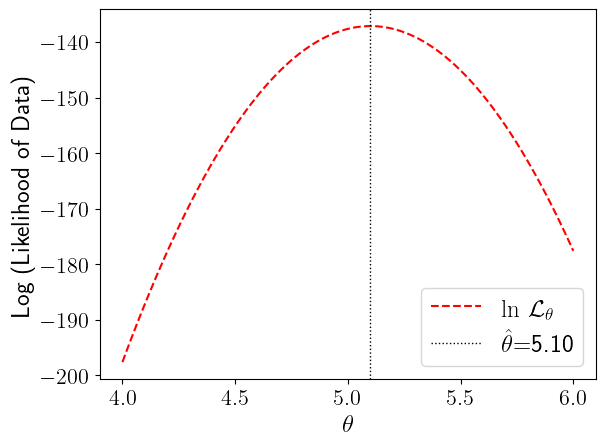
\includegraphics[scale=0.4]{PLOTDAT6-LogLikevMU.png} 
\end{center}
\end{frame}


\begin{frame}{The Score}
\footnotesize


The first derivative of the Log Likelihood with respect to the parameter(s) of interest is: $\dfrac{\partial \loglike }{\partial \theta} $\gbl{*}. This is known as \magtn{The Score, s}.\\[1ex]

\gbl{*For a vector of parameters $\theta = [\theta_{(1)},\dots, \theta_{(Z)} ] $, $s = \grad{\ln{\mathcal{L}}}$.}\\[1ex]

The score is the slope (gradient) of the Log Likelihood distribution. \magtn{The closer the score is to zero, the closer the parameter is to its maximum likelihood value.}\\[1ex]



The Score is  \bhl{$s= \dfrac{\partial \loglike}{\partial \theta}  = \dfrac{1}{\like} \dfrac{\partial \like}{\partial \theta} $} \bbl{*}\\[2ex]

\notsotiny
\bbl{* Chain rule: $f(g) = \ln g$ and $g(\theta) = \like$, so $\dfrac{\partial f(g(\theta))}{\partial \theta} = \dfrac{\partial \ln g}{\partial g}\dfrac{\partial \like}{\partial \theta} = \dfrac{1}{g}\dfrac{\partial \like}{\partial \theta} =  \dfrac{1}{\like}\dfrac{\partial \like}{\partial \theta} $} \\[1ex]


\end{frame}


\begin{frame}{The Score in terms of the PDF, $f_X$}
\footnotesize
It is useful to write the score in terms of the probability distribution rather than the likelihood, because \magtn{probabilities have nice properties like $\int f_X dx = 1$}.\\

Recall $\like = \prod\limits_i^N f_{X}(x_i;\theta) $ and $\loglike = \sum\limits_i^N \ln f_{X}(x_i;\theta) $\\
\notsotiny
\begin{align*}
s = \dfrac{\partial}{\partial \theta} \loglike &= \dfrac{\partial}{\partial \theta} \sum\limits_i^N \ln f 
\hspace{2.7cm}\bbl{Adopting\;shorthand\;f \equiv  f_{X}(x_i;\theta)\; for\; aesthetic\;reasons.} \hspace{2cm}\\
&=\sum\limits_i^N \dfrac{\partial}{\partial \theta}  \ln f
=\sum\limits_i^N \dfrac{1}{f} \dfrac{\partial f}{\partial \theta}  
\hspace{1.4cm}\bbl{ Using\; chain\; rule\;and\; \dfrac{d \ln{a} }{ da } = \dfrac{1}{a}  }\\
&= N \bbl{ \dfrac{1}{N} \sum\limits_i^N \dfrac{1}{f} \dfrac{\partial f}{\partial \theta}}
= N\, \bbl{E\left[ \dfrac{1}{ f_X } \dfrac{ \partial f_X }{ \partial \theta }  \right]} 
\hspace{0.6cm}\bbl{LLN: \plim\limits_{N\to \infty}  \overline{x} =\mu}\hspace{2cm}\\
&=  \dfrac{N}{f_X} \dfrac{\partial f_X }{\partial \theta}   
\end{align*}

\footnotesize
\magtn{ We have shown} \bhl{$s=   \dfrac{N}{f_X} \dfrac{\partial f_X }{\partial \theta} $}\\[1ex]


%$\magtn{s}= \dfrac{\partial}{\partial \theta} \loglike = \dfrac{1}{\like} \dfrac{\partial \like}{\partial \theta}  = \sum\limits_i^N \dfrac{1}{f} \dfrac{\partial f}{\partial \theta} = N \dfrac{1}{f} \dfrac{\partial f}{\partial\theta}$\;\; \rbl{ [Using LLN $\plim\limits_{N\to \infty}  \overline{x} =E[X]$]} \\

%If we consider a \bbl{single measurement}, such that $\like =\prod\limits_i^N f_{Xi} = f_{Xi}  $, the score is:\\[1ex]
%
%$\bbl{s_i}= \dfrac{\partial \ln f_{Xi} }{\partial \theta} = \dfrac{1}{f_{Xi}} \dfrac{\partial f_{Xi}}{\partial \theta} $ \\

\end{frame}




\begin{frame}{Expected Value of the Score}
\footnotesize
The score can be helpfully written in terms of the PDF $f_X$: \yhl{$s = \dfrac{N}{f_X} \dfrac{\partial f_X }{\partial \theta} $} \\[1ex]

%The Score for a single measurement: $\bbl{s_i}=\dfrac{1}{f_{Xi}} \dfrac{\partial f_{Xi}}{\partial \theta} \equiv  \dfrac{1}{f} %\dfrac{\partial f}{\partial\theta}$ (shorthand $f \equiv f_{Xi})$ \\[1ex]

The Expected Value of the score is zero:\\[1ex]
\notsotiny
\begin{align*}
E[s] & = \int s\, f_X dx \hspace{1.9cm}\bbl{LOTUS: E\left[ g(x) \right] = \int g(x) f(g) dg = \int g(x) f(x) dx }\\
& = \int \dfrac{N}{f_X} \dfrac{\partial f_X }{\partial \theta} f_X dx \hspace{1.3cm}\bbl{Substituting\; result\; from\; previous\; slide,\; s = \dfrac{N}{f_X} \dfrac{\partial f_X }{\partial \theta}}\\
& = \int N \dfrac{\partial f_X}{\partial\theta}  dx  \\
& = N \dfrac{\partial }{\partial\theta}  \int  f_X  dx \hspace{1.5cm} \bbl{Switching\; \dfrac{\partial}{\partial \theta}\; and\; \int\; is\; okay\; under\; certain\; conditions}\\
& = N \dfrac{\partial }{\partial\theta}\; 1 =  0\\
\end{align*}
\footnotesize
\magtn{ We have shown} \bhl{$E \left[s \right] =  0 $}
\end{frame}



\begin{frame}{Derivative of Expected Value of the Score \footnotesize{\bhl{$s = \dfrac{N}{f_X} \dfrac{\partial f_X }{\partial \theta} $}}}
\footnotesize
This is zero, because \bhl{$E \left[s \right] =  0 $} but we can gain insight from it:\\
\notsotiny
\begin{align*}
\dfrac{\partial}{\partial \theta} E[s] 
= \dfrac{\partial }{\partial\theta} \int   s\, f_X dx  
&= \int \dfrac{\partial }{\partial\theta}\,  \left[ s\, f_X \right] dx  
\hspace{1.8cm} \bbl{Switcheroo}\\
&= \int \left[ \dfrac{\partial s}{\partial\theta} f_X + s \dfrac{\partial f_X}{\partial\theta} \right]  dx \;\;\; \
\hspace{0.7cm}\bbl{Product\; rule\; \dfrac{d}{dx} f g = \dfrac{df}{dx} g + f \dfrac{dg}{dx}  } \\
&= \int \left[ \dfrac{\partial s}{\partial\theta} f_X +  \dfrac{s^2}{N} f_X  \right]  dx \;\;\;\;
\hspace{0.8cm}\bbl{Defn.\; of\; score:  \dfrac{\partial f_X}{\partial\theta}  =   \dfrac{s\, f_X}{N} } \\
&= \int \dfrac{\partial s}{\partial\theta} f_X dx +  \int  \dfrac{s^2}{N} f_X   dx \\
&=E \left[\dfrac{\partial s}{\partial\theta} \right] + \dfrac{1}{N}E\left[s^2\right] = 0 
\hspace{0.8cm}\bbl{Because\; we\; started\; with\; zero\; \left(\dfrac{\partial}{\partial \theta} E[s] = \dfrac{\partial}{\partial \theta} 0 =0 \right) } \\
\end{align*}
\footnotesize
%Because $E[s] =0$, $\dfrac{\partial}{\partial \theta} E[s] =0$, so \\[1ex]
\magtn{ We have shown} \bhl{$-N\,E \left[\dfrac{\partial s}{\partial\theta} \right] =  E\left[s^2\right] $}

\end{frame}




\begin{frame}{The Variance of the Score}
\footnotesize
Recall the definition of The Variance of a RV: \yhl{$V[X]  = E[X^2] - E^2[X]$}\\[1ex]

\magtn{The Variance of the score is known as The Information, $\info$}:\\
\notsotiny
\begin{align*}
V[s]  &= E[s^2] - E^2[s]  \\
& = E[s^2] \hspace{2.1cm}\bbl{Because\;E[s] =0,\; so\; E^2[s] =0}\hspace{2cm}\\
& = - N\, E \left[\dfrac{\partial s}{\partial\theta} \right]  \hspace{1.3cm}\bbl{Substituting\; result\; from\; previous\; slide, -N\,E \left[\dfrac{\partial s}{\partial\theta} \right] =  E\left[s^2\right] }\\
& = - N\, E \left[\dfrac{\partial^2 \loglike}{\partial\theta^2}  \right] 
\hspace{0.8cm}\bbl{Because\;  s= \dfrac{\partial \loglike}{\partial \theta} }
\end{align*}

\footnotesize


\magtn{ We have shown} \bhl{$V[s] = - N\, E \left[\dfrac{\partial^2 \loglike}{\partial\theta^2}  \right] \equiv \info$}\\[2ex]

\notsotiny
\gbl{Note that $\mathcal{I}_{\theta} = - \, E \left[\dfrac{\partial^2 \loglike}{\partial\theta^2}  \right]   = \dfrac{\info}{N}$ is the 'Expected Information' for a single measurement. $\info$ is the 'Observed Information'.} %Our definition is the `Observed Information' for $N$ measurements: $\info = N \mathcal{I}_{\theta} $.}
\end{frame}


\section{Info \& Variance}

\begin{frame}{The Information, $\info$\hspace{2cm} \small{\bhl{$\info = - N\, E \left[\dfrac{\partial^2 \loglike}{\partial\theta^2}  \right]  $}}}
\footnotesize

\only<1>{
\magtn{The Information $\info$ is so-called because it summarises the information about the parameter that is captured in the data.} \\
}
\only<2>{
\bbl{The Information defines the ultimate limit on the accuracy of the estimator, the Minimum Variance Bound, MVB, as we shall see next.}\\[1ex]
}

\begin{multicols}{2}
\only<1>{
A large value of $\info$ corresponds to a more `peaky' (more sharply peaked) Log Likelihood distribution, such that it is possible to discriminate between close-by values of $\theta$ when estimating the maximum likelihood value,  $\hat{\theta}$.\\

\dgreen{In this plot, the Poisson has larger variance $V[K] = \lambda=5$ than the Normal $\sigma^2=1$\;\; \ding{234}}
}
\only<2>{
Note that the expectation of the second derivative is its value at the estimate:\\

 $E \left[\dfrac{\partial^2 \loglike}{\partial\theta^2}  \right]  \equiv \dfrac{d^2\ln{\mathcal{L}_{\theta}} }{d\theta^2}\bigg|_{\hat{\theta}} $\\
 
 This is always negative, because the Log Likelihood is \magtn{concave}, so the Information is always positive.\\[1ex]
 }


\begin{center}
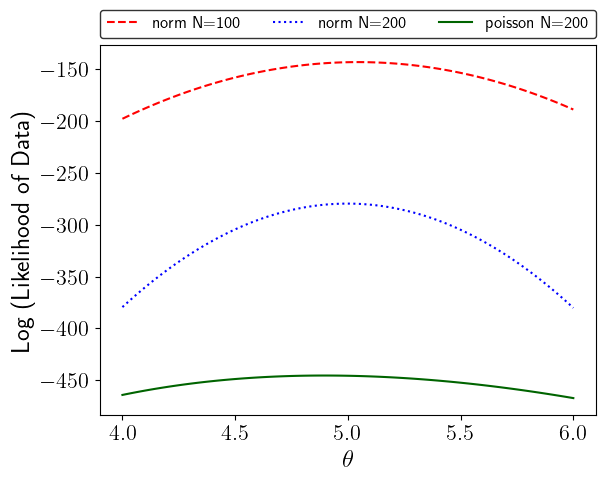
\includegraphics[scale=0.33]{Information_N100_N2200_poisson.png}
\end{center}

\end{multicols}


\end{frame}


\begin{frame}{The Hessian Matrix}
\footnotesize

If we were estimating a vector of parameters $\theta = [\theta_{1},\dots, \theta_{z} ]$, we would recover an Information Matrix, which is the negative of the \magtn{Hessian Matrix} (aka Curvature Matrix):\\[1ex]

%\magt{H_{\theta}} = 
\begin{center}
$
\magtn{H_{\theta}} =
\begin{bmatrix}
\dfrac{\partial^2 \loglike }{ \partial \rvt{1}^2} & \dots & \dfrac{\partial^2 \loglike }{ \partial \rvt{1}\partial \rvt{z} }   \\
\vdots & \ddots & \vdots \\
\dfrac{\partial^2 \loglike }{ \partial \rvt{z}\partial \rvt{1} }   & \dots &    \dfrac{\partial^2 \loglike }{ \partial \rvt{z}^2}\\
\end{bmatrix}
$
\end{center}

\vspace{0.5cm}

\bbl{Note that if we were working with the Negative Log Likelihood (convex, with a minimum), the Hessian and the Information Matrix would be identical.}

\end{frame}




\begin{frame}{The Information: Normal PDF Example}
\footnotesize
\magtn{The Log Likelihood for the Normal PDF yields the following for $\mu$:}\\[1ex]
\begin{tabular}{LL}
\loglike &= -N \ln{ \sigma} - N \ln{ \sqrt{2\pi}} - \dfrac{1}{2\sigma^2} \sum\limits_i^N (y_i-\mu)^2\\[0.5ex]
 \dfrac{\partial }{\partial \mu}  \loglike &=  \dfrac{1}{\sigma^2} \sum\limits_i^N (y_i-\mu) \hspace{1.5cm} \bbl{ First\; deriv=0\; gives\; us \;the\;MLE:\; \hat{\mu} = \overline{y}}\\[0.5ex]
 \dfrac{\partial^2 }{\partial \mu^2}  \loglike &= \dfrac{-1}{\sigma^2} \hspace{2.7cm}  \bbl{Second\;deriv\; gives\;us\;the\;information\;\info} \\[0.5ex]
\end{tabular}
\vspace{0.5cm}

\magtn{The Information is}:\\[1ex]
$\mathcal{J}_{\mu} = - N\, E \left[\dfrac{\partial^2 \loglike}{\partial\theta^2}  \right]  = -N E\left[ \dfrac{-1}{\sigma^2}\right] = \dfrac{N}{\sigma^2}$\;\;\;\bbl{ N / True Variance }\\[1ex]

\magtn{ We have shown } \bhl{$\mathcal{J}_{\mu} = \dfrac{N}{\sigma^2}$}


\end{frame}


\begin{frame}{The Information and Minimum Variance Bound}
\footnotesize

\magtn{For $Y\sim Norm(\mu,\sigma)$, the information (for $\mu$) is the inverse of the variance of the estimate $\hat{\mu}$:}  \\[1ex]

$\mathcal{J}_{\mu} = \dfrac{N}{\sigma^2}  = \dfrac{N}{V[Y]}  = \dfrac{1}{V[\overline{y}] } = \dfrac{1}{V[\hat{\mu} ]} $\notsotiny \bbl{\;\;\;\;Recall variance on the mean is $V[\overline{y}] = \dfrac{V[Y]}{N}$}\\[1ex]
\footnotesize
%:\bbl{\;\; Larger variance $\rightarrow$ Less information.}\\[1ex] 
%and the Expected Information (theoretical) is: $\mathcal{I}_{\mu} = \dfrac{1}{\sigma^2} $\\[1ex]

%$ \dfrac{N}{V[Y]} = \dfrac{1}{V[\overline{y}] } = \dfrac{1}{V[\hat{\mu}]} $ \\[1ex]

%We write $\mathcal{I}_{\mu} = \dfrac{1}{V[\hat{\mu}]}$\\[1ex]

\magtn{Generally}, the \gbl{Rao-Cramer-Frechet (RCF) Inequality} provides a \magt{Minimum Variance Bound}: the variance on an (unbiased) estimate cannot be smaller than the inverse information.\\

\begin{center}
 \ghl{$ V[\hat{\theta}] \geq  \dfrac{1}{ \mathcal{J}_{\theta} } $}
\end{center}
 If the estimator is the Minimum Variance Unbiased Estimator (MVUE, ie the best estimator!) then $V[\hat{\theta}] =\dfrac{1}{\info}$, as per the example above for Gaussian $\hat{\mu}$. \\[1ex]

%The larger the Information (more sharply peaked log likelihood), the smaller the MVB.\\[1ex]

%The (Rao-Cramer-Frechet) RCF Inequality provides a lower bound on the variance of an estimator: $V[\hat{\theta}]\geq \info^{-1}$\\

\end{frame}


\begin{frame}{The Minimum Variance Bound}
\footnotesize
The \magt{Minimum Variance Bound (MVB)} of an Estimator is the ultimate limit of its accuracy. If the Estimator is biased ($b = E[\hat{\theta}] - \theta \neq 0$) , then we must use the \gbl{full version of the RCF inequality}:\\[1ex]

 \ghl{$V[\hat{\theta}]  \geq  \left(1+ \dfrac{db}{d\theta}\right)^2\bigg/ \info $}\\[1ex]


The lower bound on the \magt{Mean Squared Error} ($MSE = V[\hat{\theta}] + b^2$) is then:\\[1ex]

\bhl{$MSE \geq  \left(1+ \dfrac{db}{d\theta}\right)^2\bigg/\info \;+\; b^2$}\\[1ex]

As we have seen, the MSE for a biased estimator can be smaller than the MSE for an unbiased one, if the biased variance is smaller than the unbiased variance.\\

\end{frame}



\section{Graphical Method}



%\section{$\ln\mathcal{L}_{\hat{\theta}} - 0.5m $}



\begin{frame}{Taylor Series Expansion of $f(x)$ about $a$}
\footnotesize
Recall the Taylor series expansion for a function $f(x)$ about the value $x=a$:\\[1ex]

\ghl{$ f(x) = \sum\limits_0^{\infty} \dfrac{f^n(a)}{n!} (x-a)^n$}\\[2ex]

%Here $f^{n}(a) \equiv \dfrac{d^nf }{dx^n}\bigg|_{x=a}$ means the $n^{th}$ derivative of the function, evaluated at $x=a$.\\[1ex]
Let's write it out in full for a few terms:\\[1ex]

$f(x) = f(a) + \dfrac{df}{dx}\bigg|_{a} (x-a) +  \dfrac{1}{2!} \dfrac{d^2f}{dx^2}\bigg|_{a} (x-a)^2 +  \dfrac{1}{3!} \dfrac{d^3f}{dx^3}\bigg|_{a} (x-a)^3+ ... $\\[1ex]


\end{frame}


\begin{frame}{Taylor Series Expansion of $\ln{\mathcal{L}_{\theta}}$ about $\hat{\theta}$}
\footnotesize

\yhl{$f(x) = f(a) + \dfrac{df}{dx}\bigg|_{a} (x-a) +  \dfrac{1}{2!} \dfrac{d^2f}{dx^2}\bigg|_{a} (x-a)^2 +  \dfrac{1}{3!} \dfrac{d^3f}{dx^3}\bigg|_{a} (x-a)^3+ ... $}\\[2ex]

Let's write this down for the Log Likelihood function, $f(x) \rightarrow \ln{\mathcal{L}_{\theta}}$, expanding about the MLE: $a \rightarrow \hat{\theta}$:\\[1ex]

$\ln{\mathcal{L}_{\theta}} = 
\ln{\mathcal{L}_{\hat{\theta}}} +
\dfrac{d\ln{\mathcal{L}_{\theta}} }{d\theta}\bigg|_{\hat{\theta}} (\theta-\hat{\theta}) +
 \dfrac{1}{2!} \dfrac{d^2\ln{\mathcal{L}_{\theta}} }{d\theta^2}\bigg|_{\hat{\theta}} (\theta-\hat{\theta})^2 + \dots
$
\vspace{1cm}
%$\loglike = \gbl{max} + \rbl{[s_{\hat{theta} \times b] }+ \bbl{\dfrac{1}{2} [\info \times b^2] }$

\magtn{Why have I stopped at the quadratic term? Lazy?}
\end{frame}




\begin{frame}{Taylor Series Expansion of $\ln{ \mathcal{L}_{\theta} }$ about $\hat{\theta}$}
\footnotesize
\begin{tikzpicture}[remember picture, overlay]
\node[xshift=-2cm,yshift=-3cm] at (current page.north east)
{
   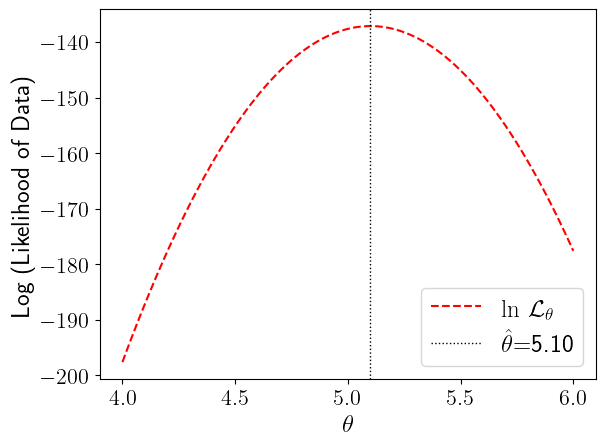
\includegraphics[scale=0.23]{PLOTDAT6-LogLikevMU.png} 
};
\end{tikzpicture}

\only<1-3>{
$\ln{\mathcal{L}_{\theta}} = 
\textcolor<1>{blue}{
\ln{\mathcal{L}_{\hat{\theta}}} 
}
+
\xxcancel<3->{
\textcolor<2>{blue}{
\dfrac{d\ln{\mathcal{L}_{\theta}} }{d\theta}\bigg|_{\hat{\theta}} 
}
(\theta-\hat{\theta}) 
}+
\dfrac{1}{2!} 
\textcolor<4>{blue}{
\dfrac{d^2\ln{\mathcal{L}_{\theta}} }{d\theta^2}\bigg|_{\hat{\theta}}
}
(\theta-\hat{\theta})^2 
$
}
\only<4>{
$\ln{\mathcal{L}_{\theta}} = 
\ln{\mathcal{L}_{\hat{\theta}}} 
+
\dfrac{1}{2!} 
\only<4>{
\textcolor{blue}{
\dfrac{d^2\ln{\mathcal{L}_{\theta}} }{d\theta^2}\bigg|_{\hat{\theta}}
}
}
(\theta-\hat{\theta})^2 
$
}

\vspace{1cm}

\uncover<1-4>{\textcolor<1>{blue}{$\ln{\mathcal{L}_{\hat{\theta}}} $}  is the maximum value of the Log Likelihood, at $\theta=\hat{\theta}$\\[1ex]}

\uncover<2-4>{
\only<2>{\textcolor{blue}{$\dfrac{d\ln{\mathcal{L}_{\theta}} }{d\theta}\bigg|_{\hat{\theta}}=0 $}
: the first derivative (score) is zero by definition at $\theta=\hat{\theta}$.\\[1ex]
}
\only<3->{\textcolor{red}{$\dfrac{d\ln{\mathcal{L}_{\theta}} }{d\theta}\bigg|_{\hat{\theta}}=0 $
: the first derivative (score) is zero by definition at $\theta=\hat{\theta}$}.\\[1ex]
}
}

\uncover<4->{
\textcolor<4>{blue}{$\dfrac{d^2\ln{\mathcal{L}_{\theta}} }{d\theta^2}\bigg|_{\hat{\theta}} $ }: the second derivative is negative (therefore not zero) for a maximum. Evaluated at $\theta=\hat{\theta}$, this is the expected value.\\[1ex]

\bbl{$\dfrac{d^2\ln{\mathcal{L}_{\theta}} }{d\theta^2}\bigg|_{\hat{\theta}} 
= E\left[\dfrac{d^2\ln{\mathcal{L}_{\theta}} }{d\theta^2}  \right] = - \dfrac{1}{V[\hat{\theta}]}$}
}


\end{frame}

\begin{frame}{Graphical Method}
\footnotesize
$\loglike = \ln\mathcal{L}_{\hat{\theta}} + \dfrac{1}{2} \dfrac{d^2\ln{\mathcal{L}_{\theta}} }{d\theta^2}\bigg|_{\hat{\theta}} (\theta-\hat{\theta})^2
=
 \ln\mathcal{L}_{\hat{\theta}} - \dfrac{1}{2} \dfrac{(\theta-\hat{\theta})^2}{V[\hat{\theta}]}
$\\[1ex]

We can now ask the question: what is the value of $\loglike$ at $\theta = \hat{\theta} \pm \sigma_{\theta}$?\\[1ex]

$
\ln{\mathcal{L}_{\hat{\theta} \pm m\sigma_{\theta}}} = 
 \ln\mathcal{L}_{\hat{\theta}} - \dfrac{1}{2} \dfrac{(\hat{\theta} \pm \sigma_{\theta}-\hat{\theta})^2}{V[\hat{\theta}]} = 
 \ln\mathcal{L}_{\hat{\theta}} - \dfrac{1}{2} \dfrac{\sigma_{\theta}^2}{V[\hat{\theta}]} =  \ln\mathcal{L}_{\hat{\theta}} - \dfrac{1}{2} 
 $\\[1ex]
 
 %The Minimum Variance Bound: $\dfrac{1}{\rm{MVB}} = \dfrac{ \sigma^2 }{N}$, so we can write:\\[1ex]
% $\ln{\mathcal{L}_{\hat{\theta} \pm m\sigma_{\theta}}} =  \ln\mathcal{L}_{\hat{\theta}} - \dfrac{m^2}{2} $

\magtn{We have shown} \bhl{$\ln{\mathcal{L}_{\hat{\theta} \pm \sigma_{\theta}}} = \ln\mathcal{L}_{\hat{\theta}} - \dfrac{1}{2} $}\\[2ex]

\bbl{ Extension to $n\sigma$ with $n>1$ is just: $\ln{\mathcal{L}_{\hat{\theta} \pm n\sigma_{\theta}}} = \ln\mathcal{L}_{\hat{\theta}} - \dfrac{n^2}{2} $}\\[1ex]
\notsotiny
%\magt{*Using Gaussian approximation: $\dfrac{1}{V[\hat{\theta}]} = \dfrac{ N }{\sigma^2}$  (only good for large $N$).}
\end{frame}



\begin{frame}{Graphical Method: Visually
\hspace{2cm}
\small{
\bhl{$\ln{\mathcal{L}_{\hat{\theta} \pm n\sigma_{\theta}}} = \ln\mathcal{L}_{\hat{\theta}} - \dfrac{n^2}{2} $}
}
}
\footnotesize


\begin{center}
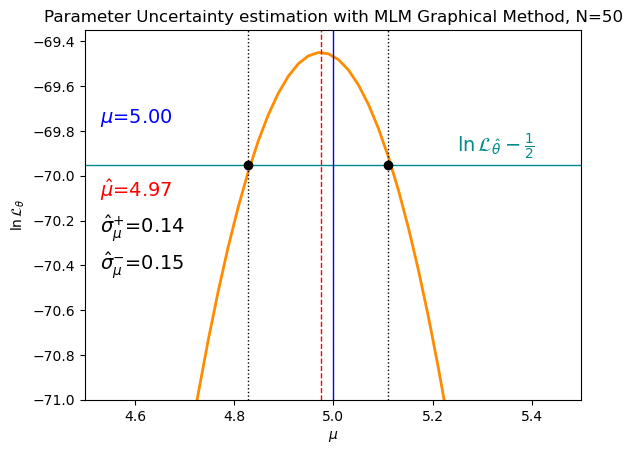
\includegraphics[scale=0.4]{PLOTDAT6-MLM-ParEst-GraphicalMethod-N50-zoom.png}
\end{center}

The graphical method is an astonishingly simple way to estimate the uncertainty on a maximum likelihood estimate. No calculus needed! The simplicity of this method is thanks to the simplicity of the shape of the log likelihood - \magtn{take care, as this is not always the case!}.\\

\end{frame}

\section{Ratio \& Wald}


\begin{frame}{MLE as an Interval Estimator}
\footnotesize

Note that the value of the Likelihood on its own is $\sim$meaningless, but a \magt{ratio} allows us to compare two models.\\[1ex]

\bhl{Likelihood Ratio:  $\lambda= \dfrac{\mathcal{L}_{\theta} }{ \mathcal{L}_{\hat{\theta}} }$}\\[1ex]

The numerator, $\mathcal{L}{_\theta}$, is for example the Likelihood for the parameter value that would correspond to our favourite theory being the correct one. Or, it could be the Likelihood for some boring null hypothesis. Either way, it cannot by definition be larger than the denominator (the maximum likelihood!), so $0\leq \lambda \leq 1$.\\[1ex]

The test statistic commonly used for the likelihood ratio is \bhl{$t_{\theta} = -2\ln  \dfrac{\mathcal{L}_{\theta} }{ \mathcal{L}_{\hat{\theta}} }$}\\[1ex]

% = -2 ( \loglike - \ln{\mathcal{L}_{\hat{\theta}}})$, therefore $ \loglike - \ln{\mathcal{L}_{\hat{\theta}}} = -\dfrac{1}{t_{\theta}}$\\[1ex]

%Recall: $\loglike = \ln\mathcal{L}_{\hat{\theta}} + \dfrac{1}{2} \dfrac{d^2\ln{\mathcal{L}_{\theta}} }{d\theta^2}\bigg|_{\hat{\theta}} (\theta-\hat{\theta})^2= \ln\mathcal{L}_{\hat{\theta}} - \dfrac{1}{2} \dfrac{(\theta-\hat{\theta})^2}{N\,\rm{MVB}}$\\[1ex]

%The smaller $t_{\theta}$ is, the better the agreement between the hypothesis $\theta$ and the data.\\[1ex]

%\magt{Wilks' Theorem} tells us that for $N\to\infty$, the PDF for the test statistic $t_{\theta}$ is $\chi^2$.\\[1ex]

\end{frame}


%\begin{frame}{Likelihood Ratio Test Statistics}
%\footnotesize
%Likelihood Ratio Test Statistic: $LR = -2 \ln{ \dfrac{\mathcal{L}_0 }{ \mathcal{L}_{\hat{\theta}} } }$\\[1ex]
%
%Wald Test: $W = \dfrac{ ( \hat{\theta} - \theta_0)^2 }{V[ \hat{\theta}] }$\\[1ex]
%
%Score (or Lagrange) Test: $S = \dfrac{s_0}{\mathcal{I}_0 }$\\[1ex]
%\end{frame}





\begin{frame}{MLE as an Interval Estimator}
\footnotesize

%Likelihood Ratio: $\lambda =  \dfrac{\mathcal{L}_{\theta} }{ \mathcal{L}_{\hat{\theta}} }$\\[1ex]

Likelihood Ratio Test Statistic: \bhl{$t_{\theta} = -2\ln \lambda =  -2\ln{\dfrac{\mathcal{L}_{\theta} }{ \mathcal{L}_{\hat{\theta}} }} = -2( \ln{\mathcal{L}_{\theta} - \ln\mathcal{L}_{\hat{\theta}} })$}\\[1ex]

% = -2 ( \loglike - \ln{\mathcal{L}_{\hat{\theta}}})$, therefore $ \loglike - \ln{\mathcal{L}_{\hat{\theta}}} = -\dfrac{1}{t_{\theta}}$\\[1ex]

Recall our conclusion from the Taylor expansion: \\[1ex]
$\loglike =  \ln\mathcal{L}_{\hat{\theta}} - \dfrac{1}{2} \dfrac{(\theta-\hat{\theta})^2}{V[\hat{\theta}]}
\;\;\rightarrow \;\;
-2( \loglike  - \ln\mathcal{L}_{\hat{\theta}} )  = \dfrac{(\theta-\hat{\theta})^2}{V[\hat{\theta}]}
$\\[1ex]

% \yhl{$\loglike = \ln\mathcal{L}_{\hat{\theta}} + \dfrac{1}{2} \dfrac{d^2\ln{\mathcal{L}_{\theta}} }{d\theta^2}\bigg|_{\hat{\theta}} (\theta-\hat{\theta})^2= \ln\mathcal{L}_{\hat{\theta}} - \dfrac{1}{2} \dfrac{(\theta-\hat{\theta})^2}{N\,MVB}$}\\[1ex]

This (approximate) likelihood ratio test statistic is called the \magt{Wald Test} and allows for the easy extraction of Confidence Intervals, as per the graphical method, in certain simple situations (PDF approximately Normal) with lots of data (large $N$).\\[1ex]

The Wald test statistic: \bhl{$W = \dfrac{(\theta-\hat{\theta})^2}{V_{_N}[\hat{\theta}]} $}\\[1ex]

\end{frame}


\begin{frame}{Wald Test, Visually}
\footnotesize
\begin{columns}
\begin{column}{0.3\textwidth}

%\only<1>{
%LR:\\[1ex] \bhl{$t_{\theta} =  -2\ln{\dfrac{\mathcal{L}_{\theta} }{ \mathcal{L}_{\hat{\theta}} }}$}\\[3ex]
%\vspace{4cm}
%}
%\only<2>{
Wald:\\[1ex] \bhl{$W = \dfrac{(\theta-\hat{\theta})^2}{V_{_N}[\hat{\theta}]} $}\\[3ex]
\vspace{4cm}
%}
\end{column}
\begin{column}{0.75\textwidth}

\begin{center}
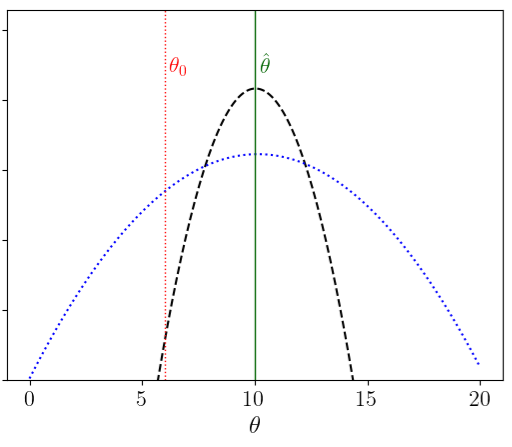
\includegraphics[scale=0.5]{wald-crop.png}
\end{center}
\end{column}
\end{columns}
\end{frame}






%We saw that \bbl{for a Gaussian}, we can write $\info = \dfrac{1}{V[\hat{\theta}]} = \dfrac{N}{\sigma^2}$, giving us $t_{\theta} = \dfrac{(\theta-\hat{\theta})^2}{\sigma^2}$.\\[1ex]



%\magtn{*Take care- like the Graphical method, this relies on large $N$, ignores `nuisance' parameters, and we have not scratched the surface regarding the matrix form of the likelihood equations!}

%We have recovered the graphical method, which allows us to find the $\pm m\sigma$ regions that can be directly converted into confidence intervals.\\

%\magtn{Wilks' theorem} (next week) tells use that in the large sample limit, the PDF for $t_{\theta}$ follows a normal $\chi^2$ distribution.\\[1ex]
 
%For a Confidence Level of $68.3\%$, we have a Confidence Interval of $\hat{\theta} \pm \sigma_{\theta}$.\\

%Recall $\chi^2 = \sum\limits_i^N \dfrac{ (\hat{\theta} - \theta)^2 }{V[\hat{\theta}]}$ 

%The smaller $t_{\theta}$ is, the better the agreement between the hypothesis $\theta$ and the data.\\[1ex]

%\magt{Wilks' Theorem} tells us that for $N\to\infty$, the PDF for the test statistic $t_{\theta}$ is $\chi^2$.\\[1ex]







%\begin{frame}{MLE as an Interval Estimator}
%\footnotesize
%
%Likelihood Ratio Test Statistic: $LR = -2 \ln{ \dfrac{\mathcal{L}_0 }{ \mathcal{L}_{\hat{\theta}} } }$\\[1ex]
%
%The numerator is the Likelihood for the Null Hypothesis $H_0$, and the denominator is the Likelihood at the estimate $\hat{\theta}$.\\
%
%Note that the value of the Likelihood on its own is meaningless, but the ratio allows us to compare two models.\\[1ex]
%
%Wald Test: $W = \dfrac{ ( \hat{\theta} - \theta_0)^2 }{V[ \hat{\theta}] }$\\[1ex]
%
%The $\theta_0$ in the numerator is the true value of the parameter according to the Null hypothesis.\\[1ex]
%
%The numerator is the squared difference between estimate and prediction, and the denominator is the variance. Exactly the form of a $\chi^2$!\\[1ex]
%The variance of the estimator is the reciprocal of the Information, which tells us about the curvature (peakiness) at the estimate.
%
%Score (or Lagrange) Test: $S = \dfrac{s_0}{\mathcal{I}_0 }$\\[1ex]
%
%
%\end{frame}




\begin{frame}{Thanks For Your Time}
\center
\Huge
Fin.
\end{frame}

\end{document}


%
%\section{Real World}
%
%
%\begin{frame}{Linking MLE to Real World Problems}
%\footnotesize
%A Loss Function aka Cost Function aka Error function is a statistic that must be minimised in order to optimise a model's description of the data.\\[1ex]
%
%For MLE, the loss function is the Negative Log Likelihood $-\loglike$\\[1ex]
%
%The Risk is the MSE: $E[ (\theta - \hat{\theta})^2]$: the expectation of the loss.\\[1ex]
%
%%$(\theta - \hat{\theta})^2$
%
%%The Expectation of the loss: $E[ (\theta - \hat{\theta})^2]$ is the Risk. This is the MSE.\\[1ex]
%
%Classification problems often use Cross-Entropy Loss: \\[1ex]
%
%$L=-\dfrac{1}{N}\sum\limits_i^N y_i \ln{\hat{y} } $\\[1ex]
%
%Regression problems often use MSE:\\[1ex]
%
%$MSE=-\dfrac{1}{N}\sum\limits_i^N (y-\hat{y})^2$\\
%
%
%\end{frame}
%
%
%
%\begin{frame}{Decision Rules}
%\footnotesize
%How to define optimality? We saw that choosing an estimator based on bias can result in a larger MSE.\\[1ex]
%
%$MSE = V+b^2$\\[1ex]
%
%Minimax argmin max R: minimizes the worst case scenario loss\\[1ex]
%
%Gradient descent is an iterative optimisation approach that gradually changes the model
%parameters to minimise a cost function 
%
%\end{frame}
%
%
%\begin{frame}{Naive Bayes}
%\footnotesize
%
%
%\end{frame}


%\only<5>{
%$\mathcal{L}_{\theta} \approx 
%\exp\left[
%\ln{\mathcal{L}_{\hat{\theta}}} 
%+
%\dfrac{1}{2!} 
%\dfrac{d^2\ln{\mathcal{L}_{\theta}} }{d\theta^2}\bigg|_{\hat{\theta}}
%(\theta-\hat{\theta})^2 
%\right]
%$
%}
%
%\only<6>{
%$\mathcal{L}_{\theta} \approx 
%\exp\left[
%\ln{\mathcal{L}_{\hat{\theta}}} 
%\right]
%\exp\left[
%\dfrac{1}{2!} 
%\dfrac{d^2\ln{\mathcal{L}_{\theta}} }{d\theta^2}\bigg|_{\hat{\theta}}
%(\theta-\hat{\theta})^2 
%\right]
%$
%}
%
%\only<7>{
%$\mathcal{L}_{\theta} \approx 
%\mathcal{L}_{\hat{\theta}}
%\exp\left[
%\dfrac{1}{2!} 
%\dfrac{d^2\ln{\mathcal{L}_{\theta}} }{d\theta^2}\bigg|_{\hat{\theta}}
%(\theta-\hat{\theta})^2 
%\right]
%$
%}
%
%\only<8>{
%$\mathcal{L}_{\theta} \approx 
%\mathcal{L}_{\hat{\theta}}
%\exp\left[
%\dfrac{1}{2!} 
%\rbl{\dfrac{d^2\ln{\mathcal{L}_{\theta}} }{d\theta^2}\bigg|_{\hat{\theta}}}
%(\theta-\hat{\theta})^2 
%\right]
%$
%}
%
%\only<9>{
%$\mathcal{L}_{\theta} \approx 
%\mathcal{L}_{\hat{\theta}}
%\exp\left[
%\dfrac{1}{2!} 
%\rbl{
%\dfrac{1}{\sigma^2}
%}
%(\theta-\hat{\theta})^2 
%\right]
%$\\[1ex]
%
%\rbl{If the Likelihood is normally distributed}, then we can see 
%\rbl{
%$
%\dfrac{d^2\ln{\mathcal{L}_{\theta}} }{d\theta^2}\bigg|_{\hat{\theta}} 
%=
%\dfrac{N}{\sigma^2}
%$
%}
%}




















%\begin{frame}{Example: Exponential PDF}
%\footnotesize
%The Exponential PDF is $f_Y(y;\lambda) = \lambda \exp[-\lambda y]$\\
%
%The Log Likelihood is $l_{\theta} = \sum\limits_i^N \ln \left[ \lambda \exp[-\lambda y_i]\right] =  \sum\limits_i^N \left[ \ln[\lambda] - \lambda y_i \right]$\\[1ex]
%
%The First Derivative wrt $\lambda$ is $\dfrac{ \partial l_{\theta}}{\partial \lambda} =  \sum\limits_i^N \left[ \dfrac{1}{\lambda} -  y_i \right]$\\[1ex]
%
%Set this to zero and solve for $\lambda = \hat{\lambda}$: \\[1ex]
%
%$\sum\limits_i^N \left[ \dfrac{1}{\hat{\lambda}} -  y_i \right] = 0\;\;\therefore\;\; \dfrac{N}{\hat{\lambda}} =\sum\limits_i^N   y_i \;\;\therefore\;\; \hat{\lambda}= N / \sum\limits_i^N   y_i $\\
%
%\magtn{Notice that this is the reciprocal of the mean: $\hat{\lambda} = \overline{y}^{-1}$}
%\end{frame}
%
%
%\begin{frame}{Example: Exponential PDF}
%\footnotesize
%The Exponential PDF is $f_Y(y;\lambda) = \lambda \exp[-\lambda y]$\\[1ex]
%The Maximum Likelihood Estimate (MLE) for the parameter $\lambda$ is $ \hat{\lambda}= N / \sum\limits_i^N   y_i $\\[2ex]
%
%The Expected Value of our MLE is:\\[1ex]
%
% $E[\hat{\lambda}] = E[N / \sum\limits_i^N   y_i ] = N E[1 / \sum\limits_i^N   y_i ] 
%= N  / \sum\limits_i^N   E[y_i]  
%= N  / ( N E[Y] ) =  1/E[Y]  = \lambda
%$\\[1ex]
%
%Where we have used  $E[y] = 1/\lambda$ for $Y\sim Expon(\lambda)$ -\magtn{recall we calculated the Expected Value and Variance for this and loads of other PDFs in week 4.}\\[1ex]
%
%\end{frame}
%
%
%
%% no leave this until we have done fisher info etc.
%\begin{frame}{Example: Exponential PDF}
%\footnotesize
%PDF: $f_Y(y;\lambda) = \lambda \exp[-\lambda y]$\\[1ex]
%MLE: $ \hat{\lambda}= N / \sum\limits_i^N   y_i $\\[1ex]
%$E[\hat{\lambda}]  = \lambda$\\[1ex]
%The Bias of the MLE is  $b = E[\hat{\lambda}] - \lambda = 0$\\[1ex]
%To check $V[\hat{\lambda}]$,  note that $\hat{\lambda} = \overline{y}^{-1}$ \\[1ex]
%\magtn{The variance}
%
%Also, $V[\overline{y}] = \dfrac{V[Y]}{N}$ and for $Y\sim Expon(\lambda)$, $V[Y] = \dfrac{1}{\lambda^2}$\\[1ex]
%$V[\overline{y}] = \dfrac{1}{N\lambda^2}$\\
%$V[\hat{\lambda} ] = \dfrac{1}{N\lambda^2}$
%\end{frame}



